%!TEX root = ../main.tex
\subsubsection{The Cantor set and the Vitali function}
Proves could require the use of counterexample to reach faster the result. Here we present two great result which can be useful to better understand the next results. First we will present the Cantor set which has quite unique characteristics in terms of its measure, then we will present a function, the Vitali--Cantor, which has interesting properties in terms of continuity and differentiation.\\
To fully understand this section the reader may read the measure chapter before, and study these results only when there is a need.

\paragraph{The Cantor set} This set has a very weird definition which leads to really useful properties, especially when they are combined in the same set. 

\begin{defn}\label{Cantor-set}
	The \emph{Cantor set} $T$ is defined as follows.\\
	Take the interval $[0, 1]$ and remove the open middle portion of size $\frac 1 3$. We call $C_1$ the remaining set: 
	$$C_1 
	\coloneqq \left[0, \frac 1 3\right] \cup \left[\frac 2 3, 1\right]
	.
	$$
	Now, from each interval of $C_1$, we remove an open middle portion of size $\frac 1 9$. Thus we obtain 
	$$
	C_2 
	\coloneqq \left[0, \frac 1 9\right] \cup \left[\frac 2 9, \frac 1 3\right] \cup \left[\frac 2 3, \frac 7 9\right] \cup \left[\frac 8 9, 1\right]
	.
	$$
	Then we iterate this process: for every $k$ we define: 
	$$
	C_k 
	\coloneqq \bigcup_{n=1}^{2^k} I_n^{(k)}
	,
	$$ where $I_n^{(k)}$ is a closed interval obtained from $C_{k-1}$ by erasing the open middle portion of size $\left( \frac 1 3 \right)^k$ from each $I_m^{k-1}$.\\
	We define the Cantor set as:
	$$
	T 
	\coloneqq \bigcap_{k=1}^\infty C_k
	.
	$$
\end{defn}

\begin{figure}[H]
	\centering
	\begin{tikzpicture}
	\newcommand{\scale}{4}
	\node[left] at (-0.3, 0) {$[0, 1]$};
	\draw (0, 0) -- (\scale, 0);
	
	\newcommand{\layers}{1}
	\node[left] at (-0.3, -\layers) {$C_1$};
	\foreach \i in {0, 2}
	\FPeval{a}{\scale * (i) / 3^\layers}
	\FPeval{b}{a + \scale / 3^\layers}
	\draw (\a, -\layers) -- (\b, -\layers);
	
	\renewcommand{\layers}{2}
	\node[left] at (-0.3, -\layers) {$C_2$};
	\foreach \i in {0, 2}
	\foreach \j in {0, 2}
	\FPeval{a}{\scale * (i + 3*j) / 3^\layers}
	\FPeval{b}{a + \scale / 3^\layers}
	\draw (\a, -\layers) -- (\b, -\layers);
	
	\renewcommand{\layers}{3}
	\node[left] at (-0.3, -\layers) {$C_3$};
	\foreach \i in {0, 2}
	\foreach \j in {0, 2}
	\foreach \k in {0, 2}
	\FPeval{a}{\scale * (i + 3*j + 9*k) / 3^\layers}
	\FPeval{b}{a + \scale / 3^\layers}
	\draw (\a, -\layers) -- (\b, -\layers);
	
	\FPeval{x}{\scale / 2}
	\node[below] at (\x, -3.2) {$\vdots$};
	\end{tikzpicture}
	\caption*{Construction of the Cantor set} % the * remove the number from the figure!
\end{figure}

The Cantor set $T$ has the following properties:
\begin{prop}\label{Cantor-set-non-empty}
	The Cantor set is non-empty, namely: $T \neq \varnothing$, and, in particular, $0, 1 \in T$.
\end{prop}
Indeed, we do not remove the extrema of each interval $I_m^{k-1}$: those extrema $0, \frac 1 9, \frac 2 9, \frac 1 3, \frac 2 3, \ldots$ are contained in $T$.

\begin{prop} \label{Cantor-set-closed}
	The Cantor set is closed.
\end{prop}
\begin{proof}
	To prove that $T$ is closed, notice that the intervals $C_k$ are closed for any $k$ as it is a finite union of closed intervals.\\
	Then, as $T$ is a countable intersection of closed set it is closed itself.
\end{proof}

\begin{prop}\label{Cantor-set-compact}
	The Cantor set is compact.
\end{prop}
\begin{proof}
	As $T$ is a subset of $\RR$, to achieve this result we have to show that $T$ is closed and bounded.\\
	It is bounded as its diameter is $1$, and it is closed as we proved the previous proposition.
\end{proof}

\begin{prop}
	The Cantor set is a Lebesgue-measurable set.
\end{prop}
To understand what this means, see definition \vref{Lebesgue-sets}.
\begin{proof}
	As $T$ is closed, it is Borel measurable as well, so it is Lebesgue measurable (see proposition \vref{Borel-sets-are-Lebesgue-sets}).
\end{proof}

\begin{prop}\label{Cantor-set-zero-measure}
	The length of the Cantor set is zero, namely $|T| = 0$.
\end{prop}
\begin{proof}
	We have $T \in C_k $ for all $k$, and thus:
	$$
	|T| 
	\le |C_k| 
	\le |\bigcup_{n=1}^{2^k} I_n^k| 
	= \sum_{n=1}^{2^k} |I_n^k| 
	= \sum_{n=1}^{2^k} \left( \tfrac 1 3 \right)^k 
	= \left( \tfrac 2 3 \right)^k
	\xrightarrow{k \to \infty} 0
	.
	$$
	So it has measure zero, and it does not contain any interval.
\end{proof}
Later, with the \textit{generalized Cantor set}, we will see that it is not necessary to have measure zero, in order to contain no intervals.

\begin{prop}\label{prop-cantor-set-perfect}
	The Cantor set $T$ is a \emph{perfect set}, namely every point $x \in T$ is a limit point for $T$. 
\end{prop}	
Equivalently we say that $T$ does not have any isolated points.
\begin{proof}
	We have to prove that for any $x \in T$ and for all $\varepsilon > 0$ we have:
	\[
	\{T \cap (x - \varepsilon, x + \varepsilon)\} \ \setminus \{x\} 
	\neq \varnothing
	\]
	
	Taking $x\in T$, by its definition we have that $x \in C_k$ for any $k \in \NN$.\\
	Then for all $k \in \NN$ there exists $n_k \in \{1, \ldots , 2^k\}$ such that $x \in I_{n_k}^k = [a_k, b_k]$.
	Recall that $|I_{n_k}^k| = \frac 1 {3_k}$.\\
	Fix $\varepsilon > 0$ and take $k$ sufficiently large so that: 
	$$
	|I_{n_k}^k|
	=(b_k -a_k)
	=\frac 1 {3^k} 
	< \varepsilon
	.
	$$
	Then $(x-\varepsilon, x + \varepsilon) \supset [a_k,b_k]$.
	Since both $a_k, b_k \in T$ we have:
	$$
	a_k, b_k 
	\in (x-\varepsilon, x+ \varepsilon) \cap T 
	\quad \forall k: 
	\quad \frac 1 {3^k} 
	< \varepsilon
	.$$
	This completes the proof.
\end{proof}

\begin{prop}\label{Cantor-set-not-contains-open-intervals}
	The Cantor set does not contain any open interval, namely: $$\mathring{T} = \varnothing.$$
\end{prop}
This prove is left to the reader, observe that each $|I_n^k|$ tends to $0$ as $k \to \infty$.

\begin{prop}\label{prop-cantor-set-uncountable}
	The Cantor set is uncountable.
\end{prop}	
\begin{proof}
	Rename each interval with \texttt{L}, \texttt{R} as follows:

	\begin{figure}[htpb]
		\centering
		\tikzset{every picture/.style={line width=0.75pt}} %set default line width to 0.75pt        

		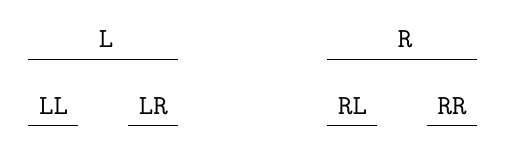
\begin{tikzpicture}[x=0.75pt,y=0.75pt,yscale=-0.8,xscale=0.8]
		%uncomment if require: \path (0,300); %set diagram left start at 0, and has height of 300

		\draw (170,120) -- (200,120);
		\draw (230,120) -- (260,120);
		\draw (350,120) -- (380,120);
		\draw (410,120) -- (440,120);
		\draw (170,80) -- (260,80);
		\draw (350,80) -- (440,80);
		\draw (211,61.4)  node [anchor=north west][inner sep=0.75pt] {$\mathtt{L}$};
		\draw (391,61.4)  node [anchor=north west][inner sep=0.75pt] {$\mathtt{R}$};
		\draw (175,101.4) node [anchor=north west][inner sep=0.75pt] {$\mathtt{LL}$};
		\draw (415,101.4) node [anchor=north west][inner sep=0.75pt] {$\mathtt{RR}$};
		\draw (235,101.4) node [anchor=north west][inner sep=0.75pt] {$\mathtt{LR}$};
		\draw (355,101.4) node [anchor=north west][inner sep=0.75pt] {$\mathtt{RL}$};
		\end{tikzpicture}
	\end{figure}
	\FloatBarrier
	
	As $C_k = \cup_{n=1}^{2^k}I_n^k$, at each subsequent step every interval $I_n^k$ is divided into two sub-intervals, namely \texttt{R} and \texttt{L}.\\	
	Let $x \in T = \cap_{k=1}^\infty C_k$. At step one $x$ can be either in \texttt{L} or in \texttt{R}. If we take $x \in \texttt{L}$, at step two $x$ can be $x \in \texttt{LL}$ or $x \in \texttt{LR}$.\\
	We continue tracing down the intervals where $x$ lies in each $C_k$, thus getting an unique, infinite sequence of \texttt{L} and \texttt{R}.\\
	Then we define a map $f: T \to E = \{\{s_k\}_{k \in \NN} : s_k = \texttt{L} \text{ or } \texttt{R} \quad \forall k\}$.
	
	We could prove that $E$ is uncountable and $f$ is bijective: we would have $|T| = |E|$ that prove our thesis.
	
	\textit{The set $E$ is uncountable:}\\ By contradiction, suppose that $E$ is countable; then we could assign a natural number to every element of $E$:
	$$E = \{ x^{(n)} = \{s_k^{(n)}\}_{k \in \NN} : n \in \NN\}.$$
	We construct a new sequence $x = \{t_n^{(n)}\}_{n \in \NN}$  with 
	\[t_n \coloneqq
	\begin{cases}
	\texttt{L} & \text{if } s_n^{(n)} = \texttt{R} \\
	\texttt{R} & \text{if } s_n^{(n)} = \texttt{L}
	\end{cases}\]
	Clearly $x \in E$, since it is made of \texttt{R} and \texttt{L}, but $t_n \neq s_n^{(n)}$ and thus $x \neq x^{(n)}$ for all $n$. Then $E$ is uncountable.
	
	\textit{The function $f$ is injective:}\\	Let $x,y \in T$ such that $f(x) = f(y)$.\\
	By construction for any $k$ we have that $x$ and $y$ belong to the same $I_n^k$.\\
	As 
	$$
	|I_n^k| 
	= \frac 1{3^k}
	$$ 
	and 
	$$
	|x-y| 
	\leq |I_n^k| 
	= \frac 1 {3^k} 
	\quad \forall k
	,
	$$
	we gain that $x=y$ and $f$ is injective.
	
	\textit{The function $f$ is surjective:}\\
	Let $\{s_k\}_k \in E$. We have to prove that there exists $x \in T$ such that $f(x) = \{s_k\}_k$.\\
	Fix $\{s_k\}_k$ and let $I_{n_k}^k$ be the interval identified by $\{s_k\}_k$ at each step $k$.\\
	In each $k$ we can take 
	$$
	y_k 
	\in I_{n_k}^k \cap T
	, \text{ with, by construction, }
	I_{n_{k+1}}^{k+1} 
	\subset I_{n_k}^k
	.
	$$
	We can assert that $\{y_k\}$ is a fundamental sequence, indeed we have:
	$$
	d_E(y_k, y_{k+1}) 
	< |I_{n_k}^k| 
	= \frac 1 {3^k} 
	\xrightarrow{k \to \infty}
	0
	.
	$$
	Moreover, $([0,1], d_E)$ is complete, indeed it is a closed subset of a complete metric space $(\RR, d_E)$, then $\{y_k\}$ is converging to an $x \in [0,1]$.\\
	As $T$ is compact, it is closed and sequentially closed, so $x \in T$.\\
	
	We have still to prove that $f(x) = \{s_k\}_k$.\\
	By contradiction suppose that there exists a sequence $\{t_k\}_k$ and a certain $\bar k$ for which $t_{\bar k} \neq s_{\bar k}$, and suppose that $f(x) = \{t_k\}_k$.\\
	Obviously $\{t_k\}_k \neq \{s_k\}_k$, indeed we have that for all $k > \bar k$ we have $t_k \neq s_k$.\\
	So $x \in I_{m_1}^{\bar k}$ (the interval represented by $\{t_k\}_k$), but $y_{\bar k}, y_{\bar k + 1}, \ldots$ belongs to $I_{m_2}^{\bar k}$ (represented by $\{s_k\}_k$).\\
	Then we have: 
	$$
	d_E(x, y_{\bar k + p}) 
	> \frac 1 {3^{\bar k}}
	\quad \forall p
	\text{ but }
	y_k 
	\to 
	x
	\text{ as }
	d(x, y_{k+p}) 
	\xrightarrow{p \to \infty}
	0
	.
	$$
	So we have a contradiction, then $f$ is bijective and this ends the proof.		
\end{proof}

\begin{prop}\label{Cantor-set-cardinalityofRR}
	The Cantor set has the same cardinality of $\RR$ and $[0,1]$.
\end{prop}

\paragraph{The generalized Cantor set} Similarly as before, it is construct by removing at each step not a third of the previous interval but a smaller, arbitrary quantity. What we will obtain is a non-zero-measure set which still have useful characteristics.

\begin{defn}
	The \emph{generalized Cantor set} $T$ is defined as follows.\\
	Fix $\eps \in (0, 1)$ and take $C_0^\eps = I_0^{\varepsilon, 0} = [0, 1]$. \\
	We build $C_1^\eps$ by erasing the open middle portion of size $\frac \eps 3$ from $I_0^{\varepsilon, 0}$, and $C_2^\eps$ by erasing the open middle portion of size $\frac {\eps^2} 9$ from $I_0^{\varepsilon, 1}$ and $I_1^{\varepsilon, 1}$, the intervals composing $C_1^\eps$.
	
	Now iterate the process: $C_k^\eps$ is constructed removing open middle portions of size $\left( \frac \eps 3 \right)^k$ from each interval $I_n^{\varepsilon, k-1}$ of $C_{k-1}^\eps$.
	
	The \emph{generalized Cantor set} is defined as:
	$$
		T_\eps 
		= \bigcap_{k=1}^\infty C_k^\eps
	.
	$$
\end{defn}

The generalized Cantor set has many properties analogues to the Cantor set, in particular holds the following propositions:
it is non-empty (\vref{Cantor-set-non-empty}), closed (\vref{Cantor-set-closed}), compact (\vref{Cantor-set-compact}), perfect (\vref{prop-cantor-set-perfect}), does not contains any interval (\vref{Cantor-set-not-contains-open-intervals}) and is uncountable (\vref{prop-cantor-set-uncountable}) with the same cardinality of $\RR$ (\vref{Cantor-set-cardinalityofRR}).\\
Anyway its measure is not zero, indeed it is easy to compute $|T_\eps|$:
$$
\left|T_\eps\right| 
= 1 - \frac \eps 3 - 2 \frac {\eps^2} 9 - \ldots
= 1 - \sum_{k=1}^{+\infty} 2^{k-1} \left( \frac \eps 3 \right)^k
= 1 - \frac 1 2 \sum_{k=1}^{+\infty} \left( \frac {2\eps} 3 \right)^k
= \frac{3(1 - \eps)}{3 - 2\eps} 
> 0
.
$$
You can still prove that $T_\eps$ does not contain any interval: start by computing $\left|I_{n,\eps}^{(k)}\right| \to 0$.

The characteristic function of $T_\eps$, $\Ind_{T_\eps}$ is Lebesgue-integrable:
$$\int_0^1 \Ind_{T_\eps} \, \de \mu = \left|T_\eps\right|.$$ 
Observe that it is not Riemann-integrable; you reader should prove it: the interior of $T_\eps$ is $\varnothing$, its measure is zero, the lower Riemann sum converges to 0, but $\left|T_\eps\right| > 0$, and thus the upper Riemann sum converges to $\left|T_\eps\right|$.

\paragraph{The Vitali--Cantor function} This function, also known as \textit{the devil's staircase}, present many properties in terms of continuity and derivability which make it a good counterexample in many situation. Its definition does not coincide with its construction. 

\begin{defn}\label{Vitali-Cantor-function}
	The \emph{Vitali--Cantor function}, is a function $f: [0, 1] \to [0, 1]$ such that:
	\begin{itemize}
		\item $f(0) = 0$ and $f(1) = 1$;
		\item $f$ is continuous and monotone non-decreasing;
		\item $f$ is derivable almost everywhere in $[0, 1]$, with $f' = 0$ almost everywhere in $[0, 1]$.
	\end{itemize}
\end{defn}

Such function can be obtained through a limit of the following series of function:
\begin{align*}
f_0(x) = & \ x\\[1 em]
f_1(x) = &
\begin{cases}
{\tfrac 3 2} x & \text{if } x \in [0, \tfrac 1 3] \\
{\tfrac 1 2} & \text{if } x \in (\tfrac 1 3, \tfrac 2 3) \\
{\tfrac 3 2} (x - \tfrac 1 3) & \text{if } x \in [\tfrac 2 3, 1] \\
\end{cases}\\[0.5 em]
= & \begin{cases}
\frac 1 2 & \text{if } x \in [0, 1] \setminus C_1 \\
\text{linear} & \text{if } x \in C_1
\end{cases} \\[0.5 em]
= & \int_0^x g_1(t) dt \qquad \text{with} \qquad g_1(t) = \frac 3 2 \Ind_{C_1}(t)\\[1 em]
f_2(x) = &
\begin{cases}
\frac 1 2 & \text{if } x \in [\frac 1 3, \frac 2 3] \\
\frac 1 4 & \text{if } x \in [\frac 1 9, \frac 2 9]  \\
\frac 3 4 & \text{if } x \in [\frac 7 9, \frac 8 9]  \\
\text{linear} & \text{if } x \in C_2
\end{cases} \\[0.3 em]
= & \int_0^x g_2(t) dt \qquad \text{with} \qquad g_2(t) = \left( \frac 3 2 \right)^2 \Ind_{C_2}(t)\\[0.5 em]
\vdots \ &\\[0.3 em]
f_k(x) = & \int_0^x g_k(t) dt \qquad \text{with} \qquad g_k(t) = \left( \frac 3 2 \right)^k \Ind_{C_k}(t)
\end{align*}

The limit of the sequence $\{f_k\}$ is the Vitali--Cantor function, we will prove this through the following propositions. Let's see its graph:
\begin{figure}[htpb]
	\centering
	% cfr. https://tex.stackexchange.com/questions/241622/plotting-the-cantor-function
	\tikzset{
	  if/.code n args=3{\pgfmathparse{#1}\ifnum\pgfmathresult=0
	    \pgfkeysalso{#3}\else\pgfkeysalso{#2}\fi},
	  lower cantor/.initial=.3333, upper cantor/.initial=.6667, y cantor/.initial=.5,
	  declare function={
	    cantor_l(\lowerBound,\upperBound)=
	      (\pgfkeysvalueof{/tikz/lower\space cantor})*(\upperBound-\lowerBound)+\lowerBound;
	    cantor_u(\lowerBound,\upperBound)=
	      (\pgfkeysvalueof{/tikz/upper\space cantor})*(\upperBound-\lowerBound)+\lowerBound;
	    cantor(\lowerBound,\upperBound)=% fun definition
	      (\pgfkeysvalueof{/tikz/y\space cantor})*(\upperBound-\lowerBound)+\lowerBound;},
	  cantor start/.style n args=5{%
	    insert path={(#1,#3)},
	    cantor={#1}{#2}{#3}{#4}{#5}{0},
	    insert path={to[every cantor edge/.try, cantor 1 edge/.try] (#2,#4)}},
	  cantor/.style n args=6{%
	    /utils/exec=%
	      \pgfmathsetmacro\lBx{cantor_l(#1,#2)}%
	      \pgfmathsetmacro\uBx{cantor_u(#1,#2)}%
	%      \pgfmathsetmacro\y{.5*(#3+#4)},% proper definition
	      \pgfmathsetmacro\y{cantor(#3,#4)},% fun
	    style/.expanded={
	      if={#6<#5}{cantor={#1}{\lBx}{#3}{\y}{#5}{#6+1}}{},
	      insert path={
	        to[every cantor edge/.try, cantor 1 edge/.try] (\lBx,\y)
	        to[every cantor edge/.try, cantor 2 edge/.try] (\uBx,\y)},
	      if={#6<#5}{cantor={\uBx}{#2}{\y}{#4}{#5}{#6+1}}{}}}}

	\foreach \level in {0,...,2}{
	\begin{tikzpicture}[line join=round] % cantor 1 edge/.style={move to}
	  \useasboundingbox[draw, scale=4, help lines]
	    (0,0) grid[xstep=1/9, ystep=.25] (1,1);
	  \draw[thick, cantor start={0}{4}{0}{4}{\level}{0}];
	\end{tikzpicture}}
	\caption{Construction of the Vitali--Cantor function.}
\end{figure}
\FloatBarrier
as we can see, it can be considered as a fractal.

\begin{prop}\label{prop-first-vitali}
	For any $k$ we have that $f_k(0) = 0$ and $f_k(1)=1$.
\end{prop}
\begin{proof}
	Considering the properties of the defined integral, as the integral domain is reduced to a point, we have $f_k(0) = 0$.
	The other result can be computed:
	$$
	f_k(1) 
	= \int_0^1 \left( \frac 3 2 \right)^k \Ind_{C_k}(t) \, \dt 
	= \left( \frac 3 2 \right)^k |C_k| 
	= 1
	.
	$$
\end{proof}

\begin{prop}\label{prop-second-vitali}
	For any $k$ we have that $f_k$ is monotonic increasing and Lipschitz-continuous.
\end{prop}
\begin{proof}
	Observe that for any $x < y$ we have:
	$$
	|f_k(y) - f_k(x)| 
	= \abs{\int_x^y g_k(t) \, \dt} 
	= \int_x^y g_k(t) \, \dt 
	\le \left( \frac 3 2 \right)^k \abs{y-x}
	.
	$$
	This fits the Lipschitz-continuity (see definition \vref{defn-lipschitz-continuity}) and shows that it is also bounded.
\end{proof}

\begin{prop}\label{prop-third-vitali}
	The sequence is piece-wise constant.\\
	In particular if  $x \in C_k\comp$, then $f_k(x) = f_{k+m}(x)$ for all $m \in \NN$, and precisely there exists $N_x \in \NN$ such that:
	$$
	f_k(x) 
	= f_{k+m}(x) 
	= \frac{N_x}{2^k} 
	\quad \forall m \in \NN
	.
	$$
\end{prop}
\begin{proof}
	First, we prove the equality. If $x \notin C_k = \bigcup_{n=1}^{2^k} I_n^k$, then there exist $N_x$ intervals $I_n^k$ such that $I_n^k \subset [0, x]$, and $(2^k-N_x)$ intervals $I_k^n$ such that $I_n^k \subset [x, 1]$, thus
	$$f_k(x)
	= \int_0^x \left( \frac 3 2 \right)^k \Ind_{C_k}(t) \, \dt
	= \left( \frac 3 2 \right)^k N_x |I_n^k|
	= \left( \frac 3 2 \right)^k N_x  \left( \frac 1 3 \right)^k
	= \frac{N_x}{2^k}$$
	
	Now we prove the value. If $x \notin C_k$, then $x \notin C_{k+1}$: since each interval $I_n^k$ produces two intervals $I_n^{k+1}$, when we have $N_x$ intervals $I_n^k \subset [0, x]$, then we also have $2N_x$ intervals $I_n^{k+1} \subset [0, x]$. Therefore:
	$$f_{k+1}(x) = \left( \frac 3 2 \right)^{k+1} \cdot 2N_x \cdot |I_n^{k+1}| = \frac{N_x}{2^k}.$$
	Thus $f_k(x) = f_{k+1}(x)$, and by induction $f_k(x) = f_{k+m}(x) \quad \forall m \in \NN$.
\end{proof}

\begin{prop}\label{prop-fourth-vitali}
	Each complementary of a set $C_k$ can be rewritten as an union of open sets, namely:
	$$
	C_k\comp 
	= \bigcup J_n^{(k)}
	,
	$$
	where $J_n^{(k)}$ are open.\\
	Moreover, if $x \neq y$ and $x, y$ are contained in the same $J_n^{(k)}$, then $f_k(x) = f_k(y)$.
\end{prop}
\begin{proof}
	Considering the previous proposition, this follows as $x, y \notin C_k$, and $N_x = N_y$.
\end{proof}

\begin{prop}\label{prop-fifth-vitali}
	The sequence $\{f_k\}$ is fundamental with respect to $d_\infty$.
	Moreover, the limit $f$ exists, $f(0) = 0$, $f(1) = 1$ and $f$ is monotonic increasing.
\end{prop}
\begin{proof}
	Take $x \in C_k\comp$. Then $f_{k+1}(x) = f_k(x)$.\\
	By continuity of $f_k$ and $f_{k+1}$ we have:
	$$
	f_{k+1}(x) 
	= f_k(x)
	\quad \forall x \in \widebar{C_k\comp}
	.
	$$
	Take now $x \in \left( \widebar{C_k\comp} \right)\comp =  \mathring{C_k}$ instead. Then $x \in \mathring{I_n^k} = (a_k, b_k)$: we have $f_{x+1}(a_k) = f_k(a_k)$ and $f_{k+1}(b_k) = f_k(b_k)$.
	
	Using the triangular inequality and the monotonicity of $f$:
	\begin{align*}
	|f_{k+1}(x) - f_k(x)|
	&= |f_{k+1}(x) - f_{k+1}(a_k) + f_{k+1}(a_k) - f_k(x)| \\
	&\le |f_{k+1}(x) - f_{k+1}(a_k)| + |f_k(x) - f_k(a_k)| \\
	&\le (f_{k+1}(b_k) - f_{k+1}(a_k)) + (f_k(b_k) - f_k(a_k)) \\
	&= 2 \cdot (f_k(b_k) - f_k(a_k))\\
	&= 2 \int_{a_k}^{b_k} g_k(t) \,\dt\\
	&= 2 \int_{a_k}^{b_k} \left( \frac 3 2 \right)^k \, \dt\\
	&= 2 \cdot \left( \frac 3 2 \right)^k \cdot \frac{1}{3^k}\\
	&= \frac{1}{2^{k-1}}
	\end{align*}
	And thus:
	\[
	d_\infty(f_{k+1}, f_{k}) 
	\le \frac{1}{2^k-1} 
	\xrightarrow{k \to +\infty} 0
	.
	\]
	Hence $\{ f_k \}$ is a fundamental sequence in $(\Cc^0([0, 1]), d_\infty)$, which is complete, and thus there exists
	$$
	f 
	\in \Cc^0([0, 1]):
	f_k 
	\xrightarrow{d_\infty} f
	.
	$$
	Thus $f(0) = 0$, $f(1) = 1$ and $f$ is monotonic increasing.
\end{proof}

\begin{prop}\label{prop-sixth-vitali}
	The function $f$ is differentiable almost everywhere; where that is possible we have $f'(x) = 0$.
\end{prop}
\begin{proof}
	Let $x \notin T$. Then there exists $k \in \NN$ such that $x \notin C_k$.\\
	But $C_k\comp$ is open, and hence there exists $\eps > 0$ such that $(x - \eps, x + \eps) \in C_k\comp$. Therefore, by what we proved in the previous points (\vref{prop-third-vitali} and \vref{prop-fourth-vitali}), we have that 
	$$
	f_{k+m}(y) 
	= \frac{N_x}{2^k}
	\quad \forall y \in (x - \eps, x + \eps) 
	\quad \forall m \in \NN
	.
	$$
	
	As $m \to + \infty$, we obtain 
	$$
	f(y) 
	= \frac{N_x}{2^k} 
	\quad \forall y \in (x - \eps, x + \eps)
	.
	$$
	This means that $f$ is constant in a neighborhood of $x$, and thus it is differentiable in $x \in T\comp$, with $f'(x) = 0$. Observe that the function $f$ is not differentiable only in $T$: but as $|T| = 0$ we have that $f$ is differentiable almost everywhere.
\end{proof}